% =====================================================================
%  CARA DRIVER COMPANION DC-1 — QUICK START GUIDE (ONE A4 PAGE)
%  Course : Electronic Product Development (Sessional) — Lab, Group 7
%  Follows: IEC/IEEE 82079-1 (task-oriented, safety first, plain language),
%           ISO 7010 / IEC 60417 style symbols, ANSI Z535.6 / ISO 3864.
%
%  BEFORE PRINTING
%  * Fill in the four FILL-IN FIELDS below. Empty link fields print a
%    dashed "QR code" box; a filled one prints the real QR code.
%  * Put the photos in the photos/ folder with the names in
%    PHOTO_SHOT_LIST.md. A missing photo prints a dashed frame.
%  * Compile with pdflatex twice. It MUST stay on one page
%    (pdfinfo shows "Pages: 1").
% =====================================================================
\documentclass[10pt,a4paper]{article}
\usepackage[a4paper,top=8mm,bottom=8mm,left=9mm,right=9mm]{geometry}
\usepackage[T1]{fontenc}
\usepackage{helvet}
\renewcommand{\familydefault}{\sfdefault}
\usepackage{amssymb,graphicx,etoolbox}
\usepackage[table]{xcolor}
\usepackage{tikz}
\usetikzlibrary{arrows.meta,shapes.geometric,positioning,calc}
\usepackage[most]{tcolorbox}
\usepackage{tabularx,array,enumitem,qrcode}
\usepackage[hidelinks]{hyperref}
\pagestyle{empty}
\setlength{\parindent}{0pt}
\setlength{\parskip}{2pt}

\definecolor{NavyBlue}{RGB}{31,56,100}
\definecolor{LightBlue}{RGB}{220,230,241}
\definecolor{WarnYellow}{RGB}{255,204,0}
\definecolor{Amber}{RGB}{242,179,61}

% ---------- FILL-IN FIELDS (leave empty until you have them) ----------
\newcommand{\Website}{https://ahmed12-stack.github.io/driver-companion_EPD/}  % product website (GitHub Pages)
\newcommand{\SupportMail}{cara.support.dc1@gmail.com}  % support e-mail
\newcommand{\VideoURL}{https://ahmed12-stack.github.io/driver-companion_EPD/video.html}  % opens the video on the website; change the video there, not here
\newcommand{\AppURL}{https://ahmed12-stack.github.io/driver-companion_EPD/downloads/driver-companion.apk}

% ---------- DOCUMENT FIELDS ----------
\newcommand{\Brand}{CARA}
\newcommand{\AppName}{Driver Companion} % the app's name on the phone
\newcommand{\ProductName}{CARA Driver Companion}
\newcommand{\ModelNo}{DC-1}
\newcommand{\DocNo}{EPD/QSG/2024-28/G07}
\newcommand{\DocRev}{1.0}
\newcommand{\IssueDate}{November 2026}

% ---------- HELPERS ----------
% Prints the value, or a marked gap when the field is still empty.
\newcommand{\field}[2]{\ifdefempty{#1}{\textcolor{NavyBlue!70}{[#2 --- to be added]}}{\expandafter\nolinkurl\expandafter{#1}}}
% QR code of a link, or a dashed box until the link is filled in.
\newcommand{\qrslot}[3]{\ifdefempty{#1}%
 {\tikz\node[draw=NavyBlue!70,dashed,line width=0.6pt,fill=LightBlue!45,minimum width=#2,minimum height=#2,
   align=center,font=\tiny\color{NavyBlue},inner sep=1pt]{\textbf{QR CODE}\\[1pt]#3};}%
 {\qrcode[height=#2]{#1}}}
% A photo from photos/, or a dashed frame naming the photo still needed.
\newcommand{\photo}[4]{\IfFileExists{photos/#1}%
 {\includegraphics[width=#2,height=#3,keepaspectratio]{photos/#1}}%
 {\tikz\node[draw=NavyBlue!60,dashed,fill=LightBlue!35,minimum width=#2,minimum height=#3,align=center,
   font=\scriptsize\color{NavyBlue}]{\textbf{PHOTO}\\#4\\[1pt]\texttt{\tiny photos/\detokenize{#1}}};}}

% ---------- SYMBOLS (drawn, ISO 7010-style) ----------
\newcommand{\warnsym}[1][0.55cm]{\begin{tikzpicture}[baseline=-0.1ex]
 \fill[WarnYellow,draw=black,line width=0.6pt,rounded corners=1pt] (0,0)--(#1,0)--(#1/2,#1*0.87)--cycle;
 \node[font=\bfseries\scriptsize] at (#1/2,#1*0.3) {!};\end{tikzpicture}}
\newcommand{\elecsym}[1][0.55cm]{\begin{tikzpicture}[baseline=-0.1ex]
 \fill[WarnYellow,draw=black,line width=0.6pt,rounded corners=1pt] (0,0)--(#1,0)--(#1/2,#1*0.87)--cycle;
 \fill[black] (#1*0.55,#1*0.68)--(#1*0.33,#1*0.34)--(#1*0.48,#1*0.34)--(#1*0.40,#1*0.12)--(#1*0.68,#1*0.45)--(#1*0.52,#1*0.45)--cycle;
 \end{tikzpicture}}
\newcommand{\hotsym}[1][0.55cm]{\begin{tikzpicture}[baseline=-0.1ex]
 \fill[WarnYellow,draw=black,line width=0.6pt,rounded corners=1pt] (0,0)--(#1,0)--(#1/2,#1*0.87)--cycle;
 \foreach \x in {0.36,0.5,0.64}{\draw[line width=0.5pt] (#1*\x,#1*0.15) .. controls (#1*\x+0.04,#1*0.3) and (#1*\x-0.04,#1*0.4) .. (#1*\x,#1*0.55);}
 \end{tikzpicture}}
\newcommand{\phonesym}[1][0.5cm]{\begin{tikzpicture}[baseline=-0.5ex]
 \draw[red!80!black,line width=1.3pt,fill=white] (0,0) circle (#1/2);
 \draw[rounded corners=0.8pt,line width=0.6pt] (-#1*0.13,-#1*0.24) rectangle (#1*0.13,#1*0.24);
 \draw[red!80!black,line width=1.3pt] (-#1*0.35,#1*0.35)--(#1*0.35,-#1*0.35);\end{tikzpicture}}
\newcommand{\weeesym}[1][0.5cm]{\begin{tikzpicture}[baseline=0pt,scale=#1/0.5cm]
 \draw[line width=0.6pt] (0.1,0.05) rectangle (0.4,0.32);\draw[line width=0.6pt] (0.05,0.32)--(0.45,0.32);
 \draw[line width=0.6pt] (0.2,0.32) arc(180:0:0.05);
 \draw[line width=0.8pt,red] (0,0)--(0.5,0.5);\draw[line width=0.8pt,red] (0,0.5)--(0.5,0);
 \fill (0,-0.12) rectangle (0.5,-0.04);\end{tikzpicture}}
\newcommand{\stepno}[1]{\tikz[baseline=-0.6ex]\node[circle,fill=NavyBlue,text=white,inner sep=1.6pt,font=\bfseries\small]{#1};}
\newcommand{\callout}[1]{\tikz[baseline=-0.6ex]\node[circle,draw=NavyBlue,fill=white,text=NavyBlue,inner sep=1pt,font=\bfseries\scriptsize]{#1};}
\newcommand{\spk}{\tikz[baseline=-0.5ex]{\fill[NavyBlue] (0,-0.06) rectangle (0.07,0.06);\fill[NavyBlue] (0.07,-0.06)--(0.16,-0.13)--(0.16,0.13)--(0.07,0.06)--cycle;
 \draw[NavyBlue,line width=0.5pt] (0.21,-0.07) arc(-40:40:0.11);}}
\newcommand{\sdot}[1]{\tikz[baseline=-0.5ex]\fill[#1] (0,0) circle (0.08cm);}
\newcommand{\say}[1]{``\textit{#1}''}

% ---------- SECTION HEADING BOX ----------
\newtcolorbox{qbox}[2][]{enhanced,colback=white,colframe=NavyBlue,boxrule=0.6pt,arc=2pt,
  fonttitle=\bfseries\small,title={#2},coltitle=white,colbacktitle=NavyBlue,
  left=3pt,right=3pt,top=2pt,bottom=2pt,boxsep=1pt,toptitle=1pt,bottomtitle=1pt,#1}

\begin{document}
\renewcommand{\baselinestretch}{1.08}\small
% ================= HEADER BAND =================
\begin{tcolorbox}[enhanced,colback=NavyBlue,colframe=NavyBlue,arc=3pt,left=6pt,right=6pt,top=3pt,bottom=3pt]
{\color{white}\begin{tabularx}{\linewidth}{@{}X r@{}}
{\large\bfseries \ProductName\ --- Quick Start Guide} & {\footnotesize Model \ModelNo\ $|$ \DocNo\ Rev \DocRev}\\
{\footnotesize Read the \textbf{Safety essentials} (E) before first use. Full details: see the \emph{Full User Manual}.} & {\footnotesize English}
\end{tabularx}}
\end{tcolorbox}
\vspace{-3pt}

% ================= ROW 1 =================
\begin{minipage}[t]{0.485\linewidth}\vspace{0pt}
\begin{qbox}{A \ \ What is in the box}
\begin{tabularx}{\linewidth}{@{}X X@{}}
$\square$ \Brand\ \ModelNo\ unit $\times$1 & $\square$ Quick Start Guide\\
$\square$ Power cable (fitted) & $\square$ Full User Manual\\
\end{tabularx}\par
{\scriptsize\renewcommand{\baselinestretch}{1}\selectfont Not supplied: power bank (5\,V, 2.4\,A or more) or car USB charger; Android phone (8.0 or newer).\par}
\end{qbox}
\vspace{2pt}
\begin{qbox}{B \ \ Know your product}
\begin{center}
\photo{qsg_front.jpg}{0.485\linewidth}{3.6cm}{Front}\hfill\photo{qsg_back.jpg}{0.47\linewidth}{3.6cm}{Back}\\[-1pt]
{\scriptsize\textbf{Front} \hspace{0.36\linewidth} \textbf{Back}}
\end{center}
\vspace{-4pt}
{\scriptsize \callout{1} Camera window \ \callout{2} Speaker \ \callout{3} PAIR button (sticker \emph{WORK})\\ \callout{4} TRIP button (sticker \emph{TO DO}) \ \callout{5} Power cable, USB-A plug}
\end{qbox}
\end{minipage}\hfill
\begin{minipage}[t]{0.485\linewidth}\vspace{0pt}
\begin{qbox}{C \ \ Set up in 4 steps}
\renewcommand{\arraystretch}{1.0}
\begin{tabular}{@{}>{\centering\arraybackslash}m{0.55cm} >{\raggedright\arraybackslash}m{\dimexpr\linewidth-3.6cm\relax} >{\centering\arraybackslash}m{2.2cm}@{}}
\stepno{1} & \textbf{Connect power.} Plug the power cable \callout{5} into a power bank. Wait about 1~min for \say{System ready.} &
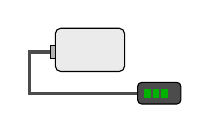
\begin{tikzpicture}[scale=0.55]\draw[rounded corners=2pt,fill=black!8] (0,0) rectangle (1.6,1);\draw[fill=black!30] (-0.12,0.3) rectangle (0,0.6);
 \draw[line width=1.2pt,black!70] (-0.12,0.45)--(-0.6,0.45)--(-0.6,-0.5)--(1.9,-0.5);\draw[rounded corners=1.5pt,fill=black!70] (1.9,-0.75) rectangle (2.9,-0.25);
 \fill[green!70!black] (2.05,-0.6) rectangle (2.2,-0.4);\fill[green!70!black] (2.25,-0.6) rectangle (2.4,-0.4);\fill[green!70!black] (2.45,-0.6) rectangle (2.6,-0.4);\end{tikzpicture}\\[18pt]
\stepno{2} & \textbf{Install the app.} Install the \AppName\ app (code in F) and allow its four permissions. &
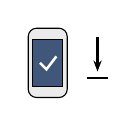
\begin{tikzpicture}[scale=0.55]\draw[rounded corners=3pt,fill=black!8] (0,0) rectangle (0.9,1.6);\draw[fill=NavyBlue!85] (0.1,0.25) rectangle (0.8,1.35);
 \draw[white,line width=0.9pt] (0.27,0.8)--(0.42,0.65)--(0.65,0.95);\draw[line width=1pt,-{Stealth[length=1.4mm]}] (1.6,1.4)--(1.6,0.6);\draw (1.35,0.45)--(1.85,0.45);\end{tikzpicture}\\[18pt]
\stepno{3} & \textbf{Pair.} Hold \callout{3} \textbf{PAIR} 5~s until \say{Pairing mode on.} Tap \textbf{Pair} in the app; type the code the unit speaks. &
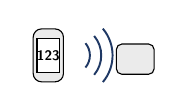
\begin{tikzpicture}[scale=0.48]\draw[rounded corners=3pt,fill=black!8] (0,0) rectangle (0.8,1.4);\draw[fill=white] (0.1,0.25) rectangle (0.7,1.15);
 \node[font=\tiny] at (0.4,0.7) {\textbf{123}};
 \foreach \r in {0.5,0.8,1.1}{\draw[NavyBlue,line width=0.7pt] (1.0,0.7)+(-40:\r) arc(-40:40:\r);}\draw[rounded corners=2pt,fill=black!8] (2.2,0.2) rectangle (3.2,1.0);\end{tikzpicture}\\[18pt]
\stepno{4} & \textbf{Drive.} Place the unit with \callout{1} facing the road. Press \callout{4} \textbf{TRIP} before you set off, and again when you park: you hear the trip summary. &
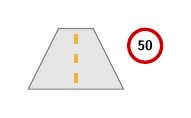
\begin{tikzpicture}[scale=0.55]\draw[fill=black!10,draw=black!50] (0,0)--(0.7,1.4)--(1.5,1.4)--(2.2,0)--cycle;
 \foreach \y in {0.15,0.6,1.05}{\draw[Amber,line width=1.4pt] (1.1,\y)--(1.1,\y+0.22);}
 \draw[fill=white,draw=red!80!black,line width=1.2pt] (2.7,1.0) circle (0.38);\node[font=\tiny\bfseries] at (2.7,1.0) {50};\end{tikzpicture}\\
\end{tabular}
\end{qbox}
\vspace{4pt}
\begin{qbox}{G \ \ Tips for best results}
\begin{itemize}[leftmargin=10pt,itemsep=1pt,topsep=1pt,parsep=0pt]
\item Set up the app and volume \textbf{before} you drive; then leave the phone alone.
\item Keep the camera window \callout{1} clean and the view through the windscreen clear: dirt, glare and wipers can hide signs.
\item The phone gives the speed: keep its Location on. Overspeed warnings need a speed-limit sign read on the way.
\item In the app, choose which apps are announced and turn on \emph{Quiet mode} when you want road alerts only.
\end{itemize}
\end{qbox}
\end{minipage}

\vspace{5pt}
% ================= ROW 2 =================
\begin{minipage}[t]{0.335\linewidth}\vspace{0pt}
\begin{qbox}{D \ \ What you will hear}
\renewcommand{\arraystretch}{1.12}
\begin{tabularx}{\linewidth}{@{}>{\raggedright\arraybackslash}p{0.5\linewidth} >{\raggedright\arraybackslash}X@{}}
\scriptsize\say{Self test passed. System ready.} & \scriptsize Ready to use\\
\scriptsize\say{Pairing mode on.} & \scriptsize Waiting 2\,min for the app\\
\scriptsize\say{Trip started.} & \scriptsize You pressed TRIP\\
\scriptsize\say{Speed limit 50.} & \scriptsize A road sign was read\\
\scriptsize\say{Slow down. Speed limit 50.} & \scriptsize You are over the limit\\
\scriptsize\say{Sign alerts paused.} & \scriptsize Camera blocked or dazzled\\
\scriptsize\say{Warning: the \ldots\ stopped working.} & \scriptsize It restarts itself; if repeated, see manual\\
\end{tabularx}\\[1pt]
{\scriptsize App status: \sdot{green!60!black} connected \ \sdot{Amber} searching \ \sdot{red!75!black} disconnected}
\end{qbox}
\end{minipage}\hfill
\begin{minipage}[t]{0.37\linewidth}\vspace{0pt}
\begin{qbox}[colframe=red!70!black,colbacktitle=red!70!black]{E \ \ Safety essentials}
\footnotesize\renewcommand{\baselinestretch}{1}\selectfont
\begin{tabularx}{\linewidth}{@{}c >{\raggedright\arraybackslash}X@{}}
\warnsym & \textbf{Driver aid only.} It can miss or misread signs. Always obey the road signs and drive with full attention.\\[1pt]
\phonesym & Do not touch the phone or the unit while driving.\\[1pt]
\warnsym & Place it so it does not block your view or an airbag, and cannot slide during braking.\\[1pt]
\hotsym & Use at 0--45\,\textdegree C. Do not leave it in a parked car in the sun.\\[1pt]
\elecsym & Use a 5\,V USB source only. Do not open the case. Keep dry.\\[1pt]
\weeesym & Do not put in household waste: use an e-waste collection point.\\
\end{tabularx}
\end{qbox}
\end{minipage}\hfill
\begin{minipage}[t]{0.27\linewidth}\vspace{0pt}
\begin{qbox}{F \ \ App, help \& support}
\begin{center}
\begin{tabular}{@{}c@{\hspace{5mm}}c@{}}
\qrslot{\AppURL}{1.45cm}{app link} & \qrslot{\Website}{1.45cm}{website}\\[1pt]
\scriptsize\textbf{Get the app} & \scriptsize\textbf{Manual \& video}\\
\end{tabular}
\end{center}\vspace{-6pt}
{\scriptsize\renewcommand{\baselinestretch}{1}\selectfont
Android 8.0 or newer\\
ahmed12-stack.github.io/\\driver-companion\_EPD\\
\ifdefempty{\SupportMail}{\textcolor{NavyBlue!70}{[e-mail --- to be added]}}{\SupportMail}\\[2pt]
Restart: unplug, wait 10\,s, plug in.\par}
\end{qbox}
\end{minipage}

\vspace{5pt}
% ================= ROW 3: SET-UP VIDEO =================
\begin{tcolorbox}[enhanced,colback=LightBlue!45,colframe=NavyBlue,boxrule=0.6pt,arc=2pt,left=6pt,right=6pt,top=3pt,bottom=3pt,
  fonttitle=\bfseries\small,title={H \ \ Watch the set-up video},coltitle=white,colbacktitle=NavyBlue,toptitle=1pt,bottomtitle=1pt]
\begin{tabularx}{\linewidth}{@{}m{2.85cm} X m{4.9cm}@{}}
\qrslot{\VideoURL}{2.6cm}{set-up video\\link to come} &
{\normalsize\bfseries See it done in about 2 minutes}\par\vspace{3pt}
Point your phone camera at the code and tap the link. The video shows each step on this page: powering the unit, installing the app, pairing, placing it on the dashboard and your first drive with the trip summary.\par\vspace{3pt}
{\scriptsize Can't scan? Open \textbf{ahmed12-stack.github.io/driver-companion\_EPD} and choose \emph{Set up}.} &
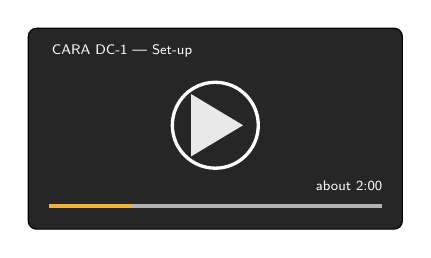
\begin{tikzpicture}[x=1cm,y=1cm,font=\scriptsize]
 \begin{scope}[scale=0.88]\draw[fill=black!85,rounded corners=3pt] (0,0) rectangle (5.4,2.9);
 \fill[white,opacity=0.9] (2.35,1.05)--(2.35,1.95)--(3.1,1.5)--cycle;
 \draw[white,line width=1.2pt] (2.7,1.5) circle (0.62);
 \fill[white!70!black] (0.3,0.3) rectangle (5.1,0.36);\fill[Amber] (0.3,0.3) rectangle (1.5,0.36);
 \node[white,anchor=north west,font=\tiny] at (0.2,2.8) {\Brand\ \ModelNo\ --- Set-up};
 \node[white,anchor=south east,font=\tiny] at (5.25,0.42) {about 2:00};\end{scope}
\end{tikzpicture}\\
\end{tabularx}
\end{tcolorbox}

\vfill
% ================= FOOTER =================
\begin{tcolorbox}[enhanced,colback=LightBlue,colframe=LightBlue,arc=2pt,left=4pt,right=4pt,top=1pt,bottom=1pt]
\scriptsize \textbf{Compliance:} educational prototype, not certified for sale; Bluetooth Low Energy, 2.4\,GHz\hfill
\textbf{Made by:} Group 7, School of Electronics Engineering, KIIT, Bhubaneswar\hfill
\DocNo\ Rev \DocRev\ \textbar\ \IssueDate
\end{tcolorbox}
\end{document}
